\documentclass[conference]{IEEEtran}
\IEEEoverridecommandlockouts
\usepackage[ngerman]{babel}
% The preceding line is only needed to identify funding in the first footnote. If that is unneeded, please comment it out.
\usepackage{cite}
\usepackage{amsmath,amssymb,amsfonts}
\usepackage{algorithmic}
\usepackage{graphicx}
\usepackage{textcomp}
\usepackage{xcolor}
\usepackage{setspace}
\usepackage{booktabs}
\usepackage[export]{adjustbox}
\def\BibTeX{{\rm B\kern-.05em{\sc i\kern-.025em b}\kern-.08em
    T\kern-.1667em\lower.7ex\hbox{E}\kern-.125emX}}
\begin{document}

\title{Currency Exchange eine App zur Anzeige von Wechselkursen mit Hilfe eines Webscrapers}


\author{\IEEEauthorblockN{1\textsuperscript{st} Matz, Annika}
\IEEEauthorblockA{\textit{dept. name of organization (of Aff.)} \\
\textit{name of organization (of Aff.)}\\
Berlin, Deutschland \\
s\_matz22@stud.hwr-berlin.de}
\and
\IEEEauthorblockN{2\textsuperscript{nd} Liebenberg, Benjamin}
\IEEEauthorblockA{\textit{dept. name of organization (of Aff.)} \\
\textit{name of organization (of Aff.)}\\
Oranienburg, Deutschland \\
s\_liebenberg22@stud.hwr-berlin.de}
\and
\IEEEauthorblockN{3\textsuperscript{rd} Reetz, Tobias}
\IEEEauthorblockA{\textit{dept. name of organization (of Aff.)} \\
\textit{name of organization (of Aff.)}\\
Berlin, Deutschland \\
s\_reetz22@stud.hwr-berlin.de}
%Beispiel wie es aussah
%\and
%\IEEEauthorblockN{3\textsuperscript{rd} Given Name Surname}
%\IEEEauthorblockA{\textit{dept. name of organization (of Aff.)} \\
%	\textit{name of organization (of Aff.)}\\
%	City, Country \\
%	email address or ORCID}
}

\maketitle


\section{Einführung}
Das Modul Software-Engineering 2 soll den Studierenden beibringen wie eine Software entwickelt wird und welche Schritte dabei einzuhalten sind. Dazu sollen sie auch selber eine Software und andere Elemente des Softwareentwicklung, wie zum Beispiel UML-Diagrammen, erstellen. Teil dieser ist ein Paper, welches genauer auf die Entwicklung der Software eingehen soll.

\section{Idee des Projektes}
Die Idee für das Modul Software-Engineering 2 besteht aus einer Android-App, die mit Hilfe eines Webscrapers Wechselkurse erhält und Beträge der unterschiedlichen Währungen ineinander umrechnet.

\section{Projektorganisation}
Innerhalb eines Softwareentwicklungsprojekts erhalten die einzelnen Bearbeitenden verschiedene Rollen, die ihnen unterschiedliche Aufgaben zu teilen. Da in diesem Fall das Entwicklungsteam aus wenigen Personen bestand, wurde entschieden, dass jeder überall helfen und arbeiten kann. Allerdings wurde für jeden Bereich wie Organisation, Serveradministration und Logo-Design eine Person gewählt, die für diesen Bereich der Ansprechpartner ist und somit auch eine Art Verantwortlicher. 

\subsection{Organisation}
Der Bereich der Organisation wurde von Annika Matz geleitet. Sie behielt die unterschiedlichen Abgabetermine im Blick. Außerdem sorgte sie dafür, dass regelmäßig Treffen in der Gruppe statt fanden und die weiteren Entwicklungsschritte besprochen wurden.

\subsection{Serveradministration}
Der Bereich Serveradministration wurde von Benjamin Liebenberg beaufsichtigt. Da er schon viel Erfahrung auf dem Bereich hatte, konnte er ohne Probleme die Leitung dieses Bereiches übernehmen.

\subsection{Logo-Design}
Das Logo-Design wurde vo Tobias Reetz übernommen, weil er bereits im Modul Software-Engineering 1 eine Rolle im Designbereich übernommen hatte. 

\section{Anforderungen}
An die Software werden immer Erwartungen und Anforderungen gestellt. Wichtig für die Entwickelnden ist Einteilung dieser und die damit einhergehende Wichtigkeit für den Erfolg des Projekts. In diesem Projekt wurden die unterschiedlichen Anforderung in drei Kategorien unterteilt. Die Kategorisierungen beinhalten nicht funktionale, funktionale und optionale funktionale Anforderungen.

\subsection{Nicht funktionale Anforderungen}
Die nicht funktionalen Anforderungen beschreiben Nicht-Erwartungen und Nicht-Ziele an die Software, die für ein erfolgreiches Projekt nicht verfolgt werden sollen. \\\\ Hier wurde festgehalten, dass die Anwendung nicht für jede Plattform zugänglich sein soll. Des Weiteren wird eine Zweisprachigkeit der App nicht unterstützt.

\subsection{Funktionale Anforderungen}
Funktionale Anforderung beinhalten Erwartungen und Ziele an die Software, welche für ein erfolgreiches Projekt erfüllt werden müssen. \\\\ Das wichtigste Ziel für die Software ist ein lauffähige Android-Handy-Applikation. Eine weitere Anforderung ist das richtige Umrechnen der verschiedenen Währungen ineinander. Weiterhin soll immer ein tagesaktueller Wechselkurs bereit stehen. In die App sollen auch mindestens sieben Währungen eingebunden werden. Zusätzlich soll die App auch ein möglichst einfaches minimalistischen Design aufweisen. 

\subsection{Optionale funktionale Anforderungen}
Anforderungen, die für ein erfolgreiches Projekt nicht wichtig sind, aber es schön wäre sie in es einzubauen, werden zu den optionalen funktionalen Anforderungen eingeteilt. \\\\ Eine dieser ist, dass die Geldbeträge in die Anzahl an Döner umgerechnet wird, die die Nutzenden sich damit kaufen könnte. Des Weiteren wäre es schön, wenn die Nutzenden prozentuale Beträge dazurechnen lassen könnten, um zum Beispiel Trinkgeld ausrechnen zu können.

\section{Entwurf}
Wie die Software aufgebaut und strukturiert werden soll, wird in dem Entwurf fest gehalten. Dieser besteht in diesem Projekt aus zwei verschiedenen Komponenten der Systemarchitektur und einem Sequenzdiagramm. 

\subsection{Systemarchitektur}
Die Systemarchitektur beschreibt wie ein System auf gebaut ist und welche Bereiche es in diesem gibt. 

\begin{figure}[h]
	\centering
	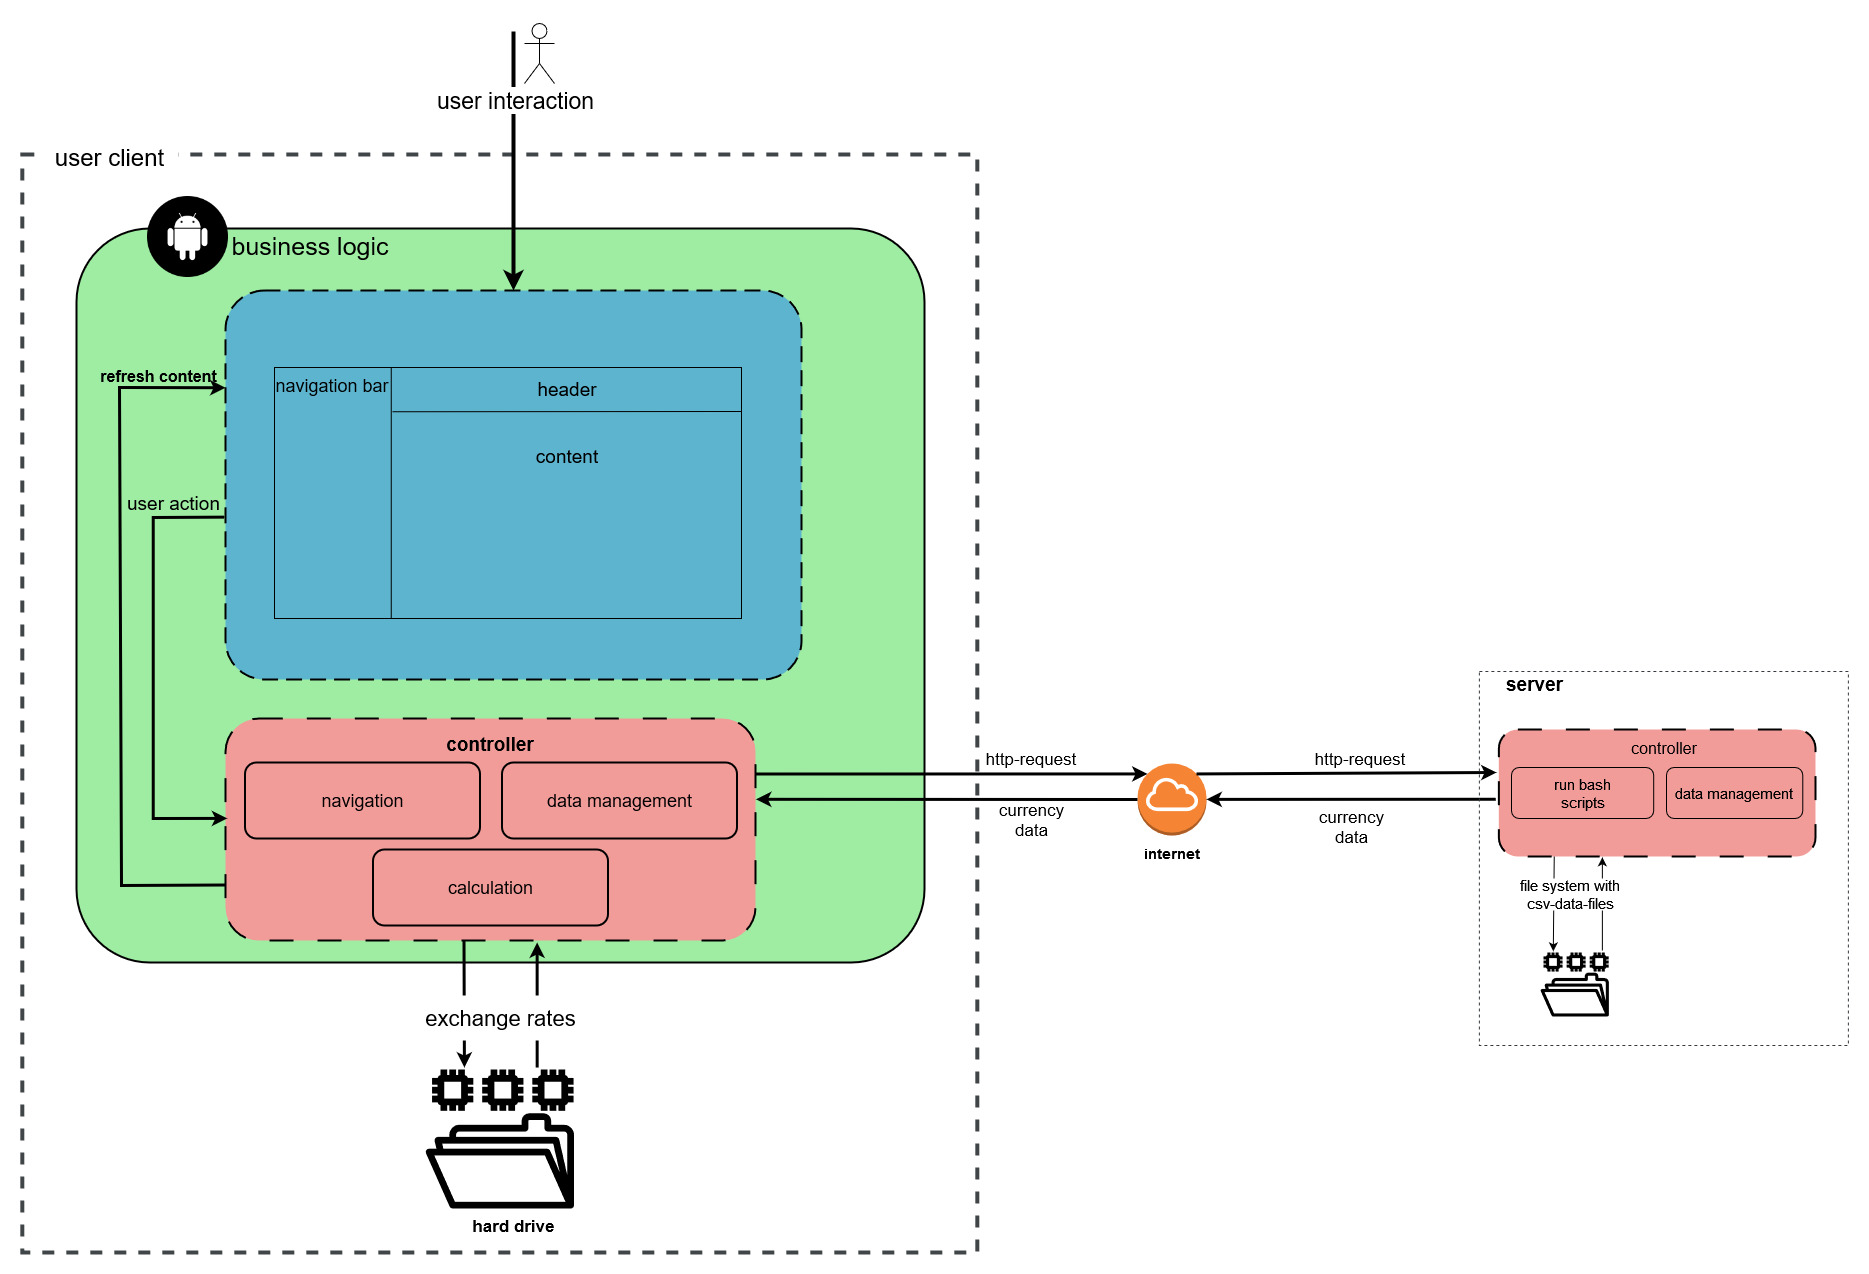
\includegraphics[width=1\linewidth, frame]{Software-Architektur_SWEII}
	\caption[Softwarearchitektur]{Softwarearchitektur}
	\label{fig:software-architektursweii}
\end{figure}
\noindent
Abbildung \ref{fig:software-architektursweii} zeigt wie die Softwarearchitektur strukturiert ist. Auf der linken Seite des Bildes ist der User-Client und auf der Rechten ist der Server. Da die Software somit zwei Komponenten aufweist, handelt es sich bei der Architektur um eine Zwei-Tier-Architektur. \\\\ Im User-Client ist zusehen, das der User mit dem in blau gekennzeichneten View interagiert. Der View ist das was die Nutzenden sehen können. Er besteht aus einem Header, einer Navigationsleiste und dem Content oder Inhalt. Über die Interaktion mit dem View können Nutzende verschiedene Controller erreichen, die im roten Bereich zu sehen sind. In dem User-Client existieren drei unterschiedliche ein mal der Navigator, der Data-Manager und der Calculator. Der Data-Manager ist dafür zuständig die Daten in einem Ordner zu speichern und sie den Anderen Controllern bereit zustellen. Er stellt auch Anfragen per HTTP-Request an den Server. Der Calculator berechnet die Wechselkurse und der Navigator sortiert Daten und stellt sie dem View bereit, der sie dann anzeigt. \\\\ Der Server weißt auch Controller auf. Er hat Bash-Skripts, die den Webscraper steuern. Der Data-Manager ist hier auch wieder für die Aufarbeitung der Daten zuständig. \\\\ Der Webscraper wurde nicht in dem User-Client integriert, da somit zu viele Anfragen auf die Webseite verhindert werden können. Sollten zu viele Anfragen an die Webseite geschickt werden, kann es zu einer Überlastung dieser kommen und sie stürzt ab. Da sie nicht Eigentum des Projektteams ist, muss dies verhindert werden, weshalb ein eigener Server zur Verfügung gestellt wird. Bei dem ist es nämlich in Ordnung, falls er überlastet sein sollte, da der Server dem Projektteam durch Benjamin Liebenberg zur Verfügung gestellt wird.

\subsection{Sequenzdiagramm}
Das Squenzdiagramm beschreibt die Kommunikation der unterschiedlichen Instanzen innerhalb der Software. \newline

\begin{figure}[h]
	\centering
	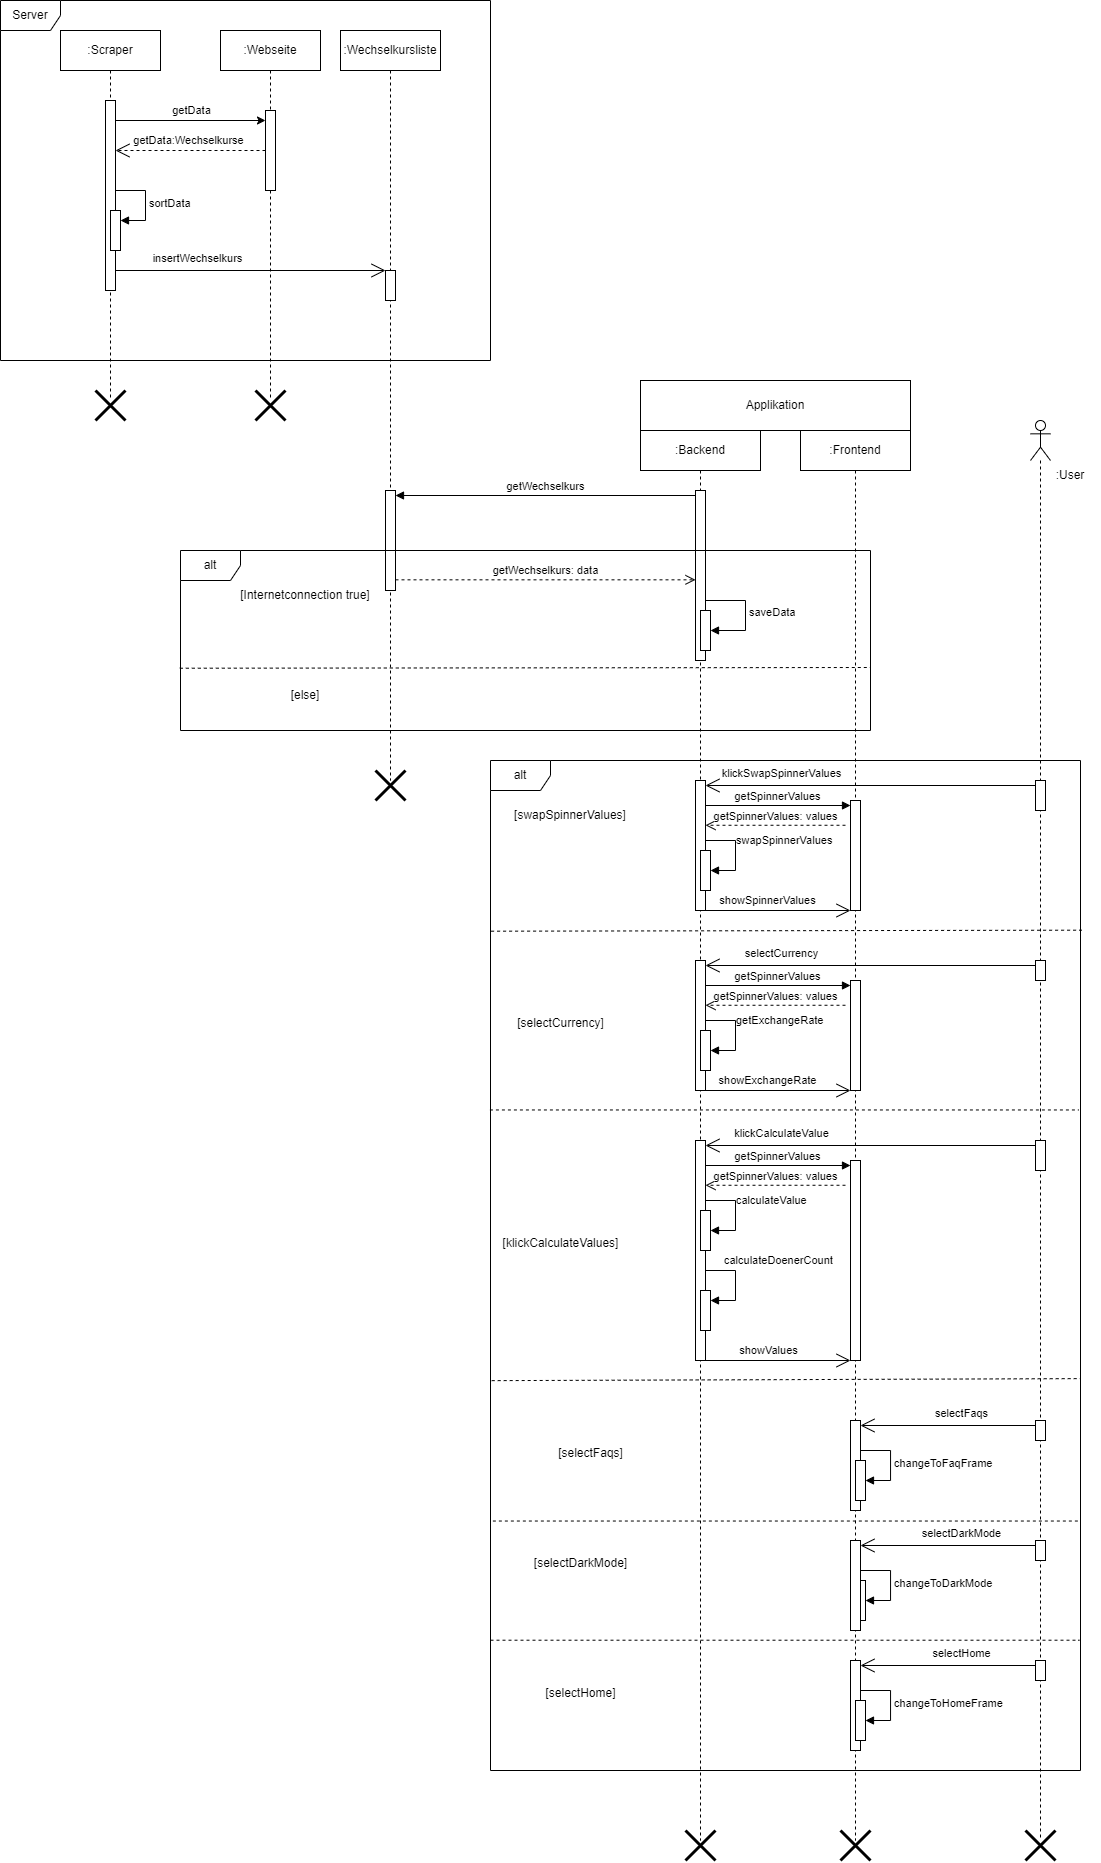
\includegraphics[width=1\linewidth, frame]{Sequenzdiagramm.drawio}
	\caption[Sequenzdiagramm]{Sequenzdiagramm}
	\label{fig:sequenzdiagramm}
\end{figure}
\noindent
Abbildung \ref{fig:sequenzdiagramm} zeigt auf, wie das Sequenzdiagramm gestaltet worden ist. Oben links ist der Serverbereich. Der Webscraper holt sich die Daten von einer Webseite und strukturiert sie. Danach werden diese dann in einer CSV-Datei gespeichert. Etwas weiter unten ist die Applikation, die wiederum in ein Front und in ein Backend geteilt ist. \\\\ Das Backend schickt eine Anfrage an den Server um die SCV-Datei zu erhalten. Sollte es eine Internetverbindung geben, erhält es diese und speichert sie ab, wenn nicht werden die Altdaten der Applikation weiter verwendet. \\\\ Unter der Abfrage ist ein alt Feld zusehen, welches alternativ Möglichkeiten der User-Applikation-Interaktion bereitstellt. Die ersten drei Optionen haben eine ähnliche Struktur. Die nutzende Person schickt eine Anfrage an das Backend. Dieses holt sich dann Daten aus dem Frontend. Danach kommen dann die Unterschiede bei den ersten drei Möglichkeiten zum Vorschein. Wenn die Werte getauscht werden sollen, tauscht das Backend die Werte. Wird eine neue Währung gewählt, sucht es den neuen Wechselkurs heraus. Soll eine Umrechnung stattfinden wird zuerst der Betrag in der Währung und dann die Anzahl der Döner berechnet. Danach sind die Möglichkeiten wieder identisch, denn das Backend schickt daraufhin eine Nachricht an das Frontend, welches die neuen Daten dann anzeigt. \\\\ Die letzten drei Möglichkeiten weisen untereinander auch wieder Ähnlichkeiten auf. Die Nutzenden schicken eine Anfrage an das Frontend, welches sich dann verändert. Die drei Möglichkeiten sind die Auswahl des Home-Seite, der FAQ-Seite und der Wechsel von und zum Dark-Mode.

\section{Implementierung}
Die Implementierung ist in drei Abschnitte geteilt. Diese Segmente sind die Implementation der App, des Servers und die Verbindung der beiden Komponenten.

\subsection{Implementierung der App}
Zur Implementierung der App wurde Android-Studio verwendet, welches eine Entwicklungsumgebung zur Entwicklung von Android-Apps ist. Innerhalb der Umgebung kann zwischen zwei Programmiersprachen gewählt werden. Diese sind Java und Kotlin. Zur Entwicklung der App wurde Java gewählt, da das Projektteam bereits Erfahrungen mit Java  durch das Modul Objekt orientierte Programmierung im zweiten Semester sammeln konnte. \\\\ Innerhalb der Java-Dateien wurde die Business-Logik implementiert. Die Darstellung der App kann auch mithilfe von Android-Studio übernommen werden. Dazu wurde in sogenannten XML-Dateien die Darstellung erstellt.

\subsection{Implementierung des Servers}
Nach der Einstellung des Servers wurde ein C\#-Skript entwickelt, welches für den Webscraper und die Datenstrukturierung zuständig ist. Es greift  auf eine Webseite zu und lädt die dortige HTML-Datei herunter. Danach liest es aus der Datei alle relevanten Daten und strukturiert diese. Nach der Strukturierung werden sie dann in einer CSV-Datei auf dem Server gespeichert. \\\\ Damit das C\#-Skript nicht jeden Tag manuell ausgeführt werden muss, wurde zusätzlich ein Bash-Skript entwickelt. Dieses Skript ist dazu zuständig jeden Tag um 6 Uhr das C\#-Skript auszuführen. \\\\ Nach der Erstellung der Skripte wurde zusätzlich eingestellt, dass die entstandene CSV-Datei über die IP-Adresse des Servers und einem Port zugänglich ist.

\subsection{Verbindung zum Server}
In der App wurde implementiert, dass sie eine Anfrage an den Port des Servers schickt, unter dem die CSV-Datei erreichbar ist. Sollte eine Internetverbindung vorliegen, wird die sie heruntergeladen und gespeichert.

\section{Integration}

\section{Tests}

\section{Wartung}

\section{Rollout}

\section{Ergebnis}

\section{Abschluss}



\end{document}
